
\documentclass[10pt,a4paper,twocolumn]{article}
\usepackage[margin=25mm]{geometry}
\usepackage{natbib}
\usepackage{url}
\usepackage[utf8]{inputenc}

\usepackage{graphicx}
\usepackage{epstopdf}
\usepackage{pdfpages}
\usepackage{tabularx}
\usepackage{float}
\usepackage{subcaption}
\usepackage{amsmath}
\usepackage{amsfonts}
\usepackage{amssymb}
\renewcommand{\familydefault}{lmr}

\begin{document}

% paper title
\title{\textbf{DashThings \\ Project in Software Customization Ubiquitous Computing}}

% author names
\author{Nikolaj Schademose Reibke, nirej666@student.sdu.dk\\Emil Sebastian R{\o}mer, emroe12@student.sdu.dk}

% make the title area
\maketitle

%\tableofcontents
\section{Introduction}
The first step towards automatization of buildings and homes with Internet of Things is to understand the data provided. 
Through this understanding it is then possible to decide actions to take based on one or more sensor input given. 
Making decisions and taking action for one building is not generalizable enough to apply to other buildings without customization. 
Further are actions rooted in a problem that needs to be solved. 
This means that customization is needed whenever one of the following is true:
\begin{itemize}
\item Problems that needs to be solved might differ from one building to  another building
\item The buildings infrastructure might not be the same between buildings meaning that the solution might differ
\item Context of the environment have changed
\end{itemize}

In general there is a great need for customization or customizable application in building  automatization through Internet of Things.

Using charts or graphs to visualize large amounts of complex data is easier than poring over the data itself. 
Data visualization is a quick, easy way to convey concepts in a universal manner. Data visualization can be used for different purposes. 
Some of these are:
\begin{itemize}
\item Decision making
\item Identify areas that need attention or improvement
\item Clarify which factors influence behaviuor
\item Identify behaviour or patterns
\end{itemize}

The problem is that a visualisation is not universal in sense of the purposes it can be used for. 
Therefore, there are a great need for customized or customizable visualizations that supports the different purposes. 

The purpose for the project is to have a website, with responsive design, which can be viewed on any browser like Mobile, Desktop, Laptop and tablet. 
The pages on the website will contain Links between the pages on the webpage. 
It will also be possible to link to external webpages. 
Additionally the pages will contain graphs and tables which shows data. 
The data will either be fetched from external sources or external sources will have the possibility to post data to a data source given a predefined data schema. 

Data in data sources can be transformed using formula expressions and have to go through at least 1 formula expression in order to be displayed on a graph. 
This expression will be on the graph. 

In order to enable the user to create the above in a easy customizable way three self made language will be used.

\section{Tools}
This Section explains what tools has been used in what part of the project and also
what external development tools has been used.

\subsection{Project Bound Tools}
Project Bound Tools is tools, frameworks and libraries required for the project to work.

\paragraph{RabbitMQ(ADD REFERENCE)(Partial)} Not fully required but should be installed
on the running server running DashThinks
\paragraph{Python 3.4+} The product generated of DashThinks is python code and all execution
has been established with Python 3.4 and newer.

addtional the following python libraries is required for the project to run:
\begin{itemize}
\item Django version 1.9.4
\item amqp 1.4.9
\item celery 3.1.23
\item django-celery 3.1.17
\item djangorestframework 3.3.3
\item numpy 1.10.4
\end{itemize}

\paragraph{Java} Java is the base for both XText and XTend to run, additionally the language
compiler is also java based code. The Java version required would be at least Java 7, but all
execution and development work has been done using the recommended Java 8.

\paragraph{A browser} is required to see the result of a program as the product of a program
is a webpage. 

\subsection{Development Process Tools}
The Process Tools are tools which contributed not directly to the developed project but was
used as process tools to contain the project.

\paragraph{Git} has been the only tool used for version control of the code.

\paragraph{LaTeX} has been the choice for writing the the project report.



\section{section1}
%\input{}

\section{The Domain Specific Language, DSL}
\subsection{Overview}
The DSL is divided into three components, a arithmetic expressions language, a language for specifying a web site and a language for specifying input sources for the system. 
The expression language is a utility language which is included by the two others. 
This language defines how a user can create arithmetic expressions in either of the other two languages. 
The Web visualizer is a language to create dynamic web sites, like the sample page shown on the front page. 
This language lets the user create pages on a site, link different pages to each other and visualize information through the use of graphs. 
The Datasources language, which is still to be developed, will be used to specify different data sources, like for instance a external databases or APIs. 
In addition this language will also be used to specify internal persistence and a API for other systems to use for posting data to the Dashk system.

\subsection{The Formula Expression Language}
The Formula Expressions DSL is responsible for understanding mathematical formulas, which will be applied to tables of data.
\paragraph{Meta model}

The formula metamodel consist of multiple elements for an overview seen in Figure
\ref{fig:formulaModel}. The types include in the elements included in the model are:
\begin{enumerate}
\item Formula: The overall Structure Element
\item Variable: The variable names included in the formula, appears both left and right side of the equation
\item Expression: The right side of the equal sign in a formula. The Expression collects the parts which is connected with plus($+$) and minus($-$). 
\item Factor: A semi-structure of the expression, Factors collects the parts connected with multiplication($\cdot$) and division($/$).
\item Op1: Identifies a addition or substraction operation
\item Op2: Identifies a multiplication or divison a operation
\item Primitiv: Identifies as either a number or a Variable
\end{enumerate}

\begin{figure}
  \begin{center}
    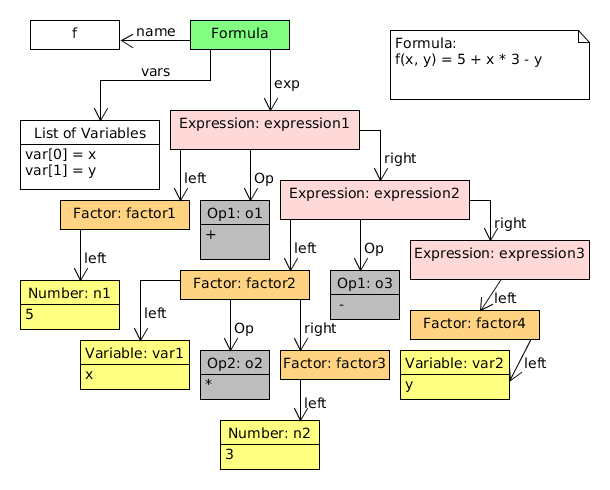
\includegraphics[width=\linewidth]{images/formulaInstance}
  \end{center}
  \caption{Instance of Formula}
  \label{fig:formulaInstance}
\end{figure}

Given the following the example: $$f(x, y) = 5 + x \cdot 3 - y$$
The rules for the grammar is explained as below also referring to
Figure \ref{fig:formulaInstance}:
\\
A Formula Contains a name which is defined as the letter/word in front of the paranthesis
also underlined in the following formula: $\underline{f}(x, y) = 5 + x \cdot 3 - y$.
In Figure \ref{fig:formulaInstance} ``f'' is defined as ``name'' seen as an attribute
for the overall Formula.
It also contains a list of variables, defined within the paranthesis seperated
by ``,'' as underlined: $f\underline{(x, y)} = 5 + x \cdot 3 - y$. The variables is saved
as a list under formula as ``vars'' seen at List of Variables.
Finally the expression of the formula is everything on the right side of the equal-sign(``=''),
here follows the rule that every variable used in the expression has to appear inside
the paranthesis on the left side of the formula as well, as it works as a function,
the expression part underlined: $f(x, y) = \underline{5 + x \cdot 3 - y}$ refered to
as ``exp'' and seen as ``expression1'' in Figure \ref{fig:formulaInstance}. 

Looking at the expression(``expression1''): $5 + x \cdot 3 - y$ it is broken down by continouisly
working from the left to the right. the left part of the expression is defined as a factor until
it meets an addition or substraction sign. For the formula example this would put only the number
``5'' into the left side factor as ``factor1'' in Figure \ref{fig:formulaInstance},
futher containing ``5'' in the Number object ``n1''.
Expression2 is then the rest of the equation after $5 +$. The new expression
contains again one factor which is the left side($x \cdot 3$) seperated by the substraction sign
The factor ``factor2'' contains on the left ``var1'' which is x, and on the right another factor
is spawned seen as ``factor3'' in Figure \ref{fig:formulaInstance}, only containing a left
side being the number seen in ``n2'' as 3.
Coming back up to the expression. it contains the last part of y as ``expression3''
which only a left side being a factor(factor4) and that factor also only contains a left side
which is the variable ``var2'' being the y.

For the variables ``var1'' and ``var2'', both is included in the List of Variables in as seen in
Figure \ref{fig:formulaInstance}


\begin{figure}
  \begin{center}
  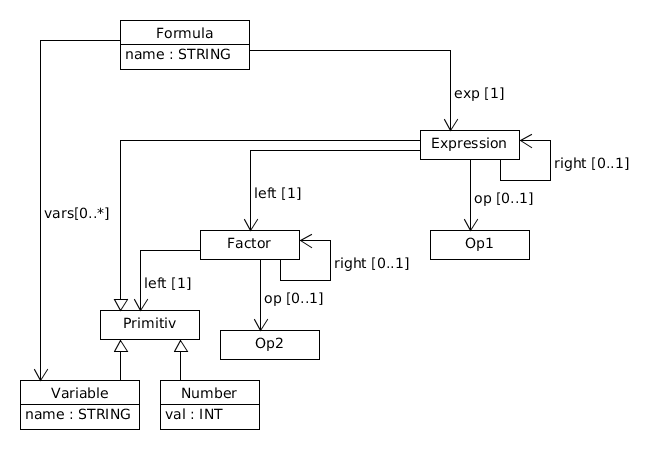
\includegraphics[width=\linewidth]{images/MetaFormula}
  \end{center}
  \caption{Model of the formula module}
  \label{fig:formulaModel}
\end{figure}
\paragraph{Language Validation}
has been archieved partly by the BNF\footnote{\cite{BNF}} using Xtext, but also
using Xtend to write additional validation code, where the Xtext language was not sufficient
to validate that the structure did indeed not violate any rules.

Xtext could only validate the general structure of the model.
what xtext was not archieved was to have xtext validate that the only variables used
on the right side og the equation sign was declared on the left side.
In order to validate that the variables on the right was declared on the left a
collection containing the declared variables on the left was matches against all the variables
on the right fetched using recursion with depth first search.

\subsection{The Web visualizer Language}
For generating dashboards custom language have been created.
This language specify:
\begin{itemize}
\item Which pages the web-interface consist of
\item The navigation between pages
\item Which data to display and where
\item Where and how to obtain the data
\subitem Internal data streams
\subitem External data streams
\item How to manipulate the data streams
\end{itemize}
The following subsection will look into detail of how the language is structured and the syntax and grammar of the language.

\subparagraph{The Grammar}
\begin{figure}
\begin{center}
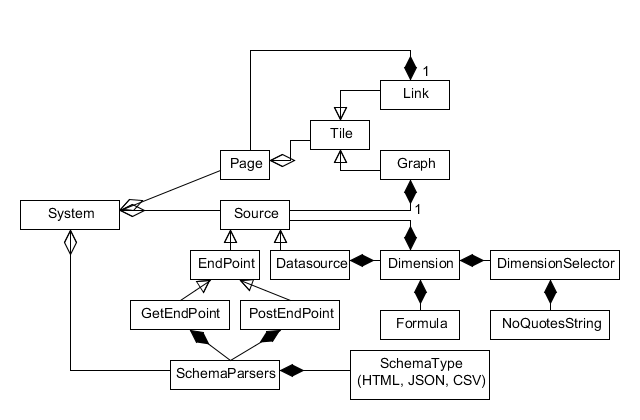
\includegraphics[width=\linewidth]{images/languagemodel}
\end{center}
\caption{Model of the language}
\label{fig:languagemodel}
\end{figure}
Figure \ref{fig:languagemodel} shows the structure of the language.
This model shows that the language defines of a system containing three parts:
\begin{itemize}
\item Pages
\item Sources
\item Schemas
\end{itemize}

\textbf{The Pages,} is what the language in turns will use to create web pages in a system defined in the language.
A page is a collection of tiles. 
Each tile is an extendible definition of a visual object on a page.
In the current version, there are two types of Tiles, Links and Graphs.
A Link definition contains a pointer to a page. 
A Graph however, has a reference data \textit{source} from witch it needs to fetch data from.
\begin{figure}
\begin{center}
\lstinputlisting[language=Java, frame=single, breaklines=true,tabsize=3]{code/GrammaDefinition.xtext}
\end{center}
\caption{Sample grammar definition, For a complete view of the grammar, see Appendix }
\label{fig:grammadefinition}
\end{figure}
Figure \ref{fig:grammadefinition} shows a sample code snippet from the grammar definition.
The Figure shows how the grammar is defined for the Pages, Tiles, Links and Graphs.
Similar does Figure \ref{fig:examplePages} show and example use of this grammar. 
This example creates a system object with two pages inter connected by links and with a number of graphs.
\begin{figure}
\begin{center}
\lstinputlisting[language=Java, frame=single, breaklines=true,tabsize=3]{code/ExampleUsePages.vis}
\end{center}
\caption{Example language use, defining pages}
\label{fig:examplePages}
\end{figure}

\textbf{The Sources, } can be of two different types, an \textit{EndPoint} or a \textit{DataSource}.
An EndPoint is intended to function as interface towards external systems or data sources. 
Whereas a Datasource is an internal definition intended for filtering, data manipulation or data grouping.\\
This Source, Endpoint, Datasource-Dimension structure have been defined as a compositional pattern, with source as the component, the Endpoint as a leaf and the Datasource as the composite.
This pattern makes the it possible to compose any number of different structures.
In addition every defined dimension comes with a formula, which will be applied to the data.
Since Source can have multiple dimensions (data streams) when specifying a how a Source an additional dimension selector can be specified to select a subset of the dimensions.
Figure \ref{fig:exampleDatasources} shows and example of a Datasource created through the language. 
The first line creates a Datasource and the declares a list of dimensions. 
Each declaration of a dimension starts by declaring a formula. After the formula follows a declaration of Sources to use in the formula. 

\begin{figure}
\begin{center}
\lstinputlisting[language=Java, frame=single, breaklines=true,tabsize=3]{code/ExampleUseDataSources.vis}
\end{center}
\caption{Example language use, defining data sources}
\label{fig:exampleDatasources}
\end{figure}

Figure \ref{fig:exampleEndpoints} is an example of the use of Endpoints.
In this, a GetEndPoint is created. This Endpoint type contains a url, a header and a schema parser.
In addition this can contain a data field used when for POST request returning data, like for instance the query language of the SMap system.
\begin{figure}
\begin{center}
\lstinputlisting[language=Java, frame=single, breaklines=true,tabsize=3]{code/ExampleUseEndPoint.vis}
\end{center}
\caption{Example language use, defining endpoints}
\label{fig:exampleEndpoints}
\end{figure}

\textbf{The Schemas,} or SchemaParsers are a global way of defining how to parse date from an external source.
This is both needed when defining an source to request data from and when external sources posts data to the system.

\paragraph{Meta model}
The language compiles a dynamic website using the Django framework.
This framework uses an MVC architektur which is extended with a template pattern with HTML documents. 
In order to make the output easy readable and customizable for a user the output needs to be mapped into a model that follows this pattern with more explicit information.

In order to do so, a meta model of the a website using this framework have been created which incorporates the functionality of the desired dashboard system.  
Figure \ref{fig:websitemodel} shows this meta model.
This meta model differs in a number of ways from the model created by the language.
This is due to the high complexity of the Django framework.
In order to keep the language simple the group decided to create a simpler model for the language (see Figure \ref{fig:languagemodel}) and map this model to the created meta model of the system.
The meta model however have adopted some aspects of the language model, like for instance the part concerning Datasources, Endpoints, parsers and selectors.
The Django framework uses a MVC pattern. 
Which means that the constructed pages and content needs to be mapped into this form.
The Django way, is to define a controller in form of a urls fils containing the mapping of urls to either views of the system or other urls files.
The views can then either use a model and/or a HTML template file to build up the responses for a request with the use of a number of serializes.

\begin{figure}
\begin{center}
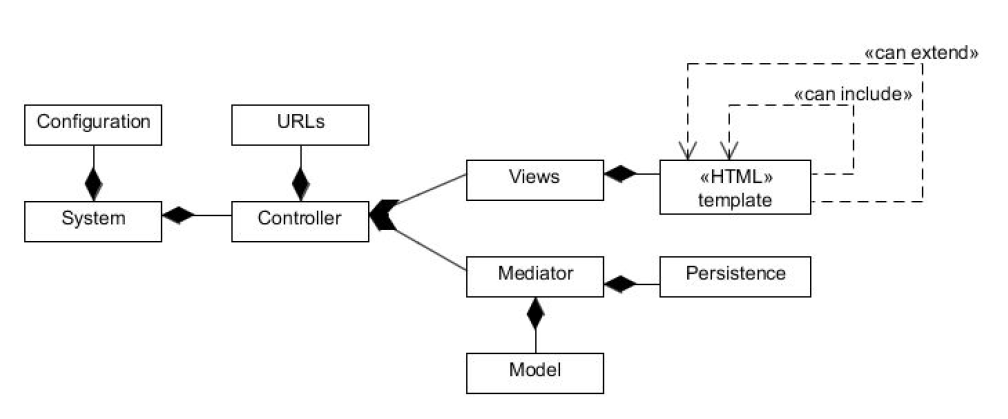
\includegraphics[width=\linewidth]{images/websitemodel}
\end{center}
\caption{Model of the Website}
\label{fig:websitemodel}
\end{figure}

\paragraph{Language Validation}
of the entire vizualizer project containing validating the following items:
\begin{enumerate}
\item \textbf{[XText]} The page linked to from one page to another existed
\item \textbf{[XText]} Graphs contains an existing reference to a Datasource
\item \textbf{[XText]} GetEndPoints contains a Schema
\item \textbf{[XText]} Schemas contain at least 1 Selector
\item \textbf{[XText]} Datasources contains at least one Dimension
\item \textbf{[XText]} Dimension contains at least one reference to a Source
\item \textbf{[XTend]} Datasources have no cyclic dependencies
\item \textbf{[XTend]} All the variables declared on the left side of a formula is also declared under one of the DimensionSelectors listed for that Dimension.
\item \textbf{[XTend]} All Datasources is directly or indirectly connected to an EndPoint
\end{enumerate}

It was not archieved to validate all the rules in the grammar strictly using XText and a few
of the rules had to be checked in the syntax tree. XText can make checks like that a reference is
existing and that the overall grammar structure is correct.
The things that XTend can do is that after the initial grammar, the instance of the grammar is
built and that gives some additional possibilities to validate the program from XTend. Here
only the full validation should be possible, given that the language is not turing
complete\footnote{make ref to turing completeness}. As listed previously cyclic dependencies
can be checked a long with more advanced type checking. Maybe a language would contain an odd
rule that the number 5 would not be allowed. This could be put into the XText document,
but would be much easier to validate using XTend. Here we could also extend the Formula projects
language validation rules within the Vizualizer language futher using XTend by checking that
declared variables on the left side of a formula was supported by a declared variable from
a DimensionSelector. 

\paragraph{Code generation}
To maintain a clean code structure all generated code are put into a number of different packages, see Figure \ref{fig:packagediagram}.
This diagram shows the structure of the generated code.
\begin{figure}
\begin{center}
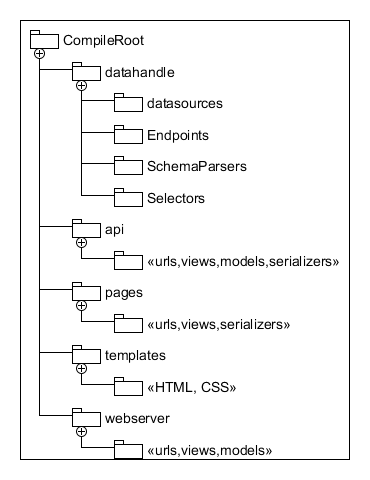
\includegraphics[width=\linewidth]{images/PackageDiagram}
\end{center}
\caption{Package diagram of generated sources}
\label{fig:packagediagram}
\end{figure}
The data handle package contains all code for handling obtaining data from external systems. 
Into here the data sources, endpoints selectors and schema parsers are generated.
The api package contains the code generated for creating a API for external sources to post data.
This package will contain  models, views, serializes and a controller for the API.
A page object from the language model is split into a number of fractions.
A page needs to be divided into a model a view, a controller and a HTML template document.
Better keep things apart the template documents have been gathered in a package by itself (the template package).
The model views and controllers are generated into the pages package.
Each page gets it own template file extending a base template file making them easy customizable.
The individual template file contains only the structure of the specific links and graphs (without data) of that page.

\subparagraph{Generation}
The code generation have been done through the [XTend] language.
This language provides some additional coding features for the plain Java language.
One of the highly used features is the multi dispatching.
Figure \ref{fig:multidispatching} how formulas are generated using multi dispatching in a nested loop.

\begin{figure}
\begin{center}
\lstinputlisting[language=Java, frame=single, breaklines=true,tabsize=3]{code/multidispatch.java}
\end{center}
\caption{Code generation with multi dispatching}
\label{fig:multidispatching}
\end{figure}


\section{section3}
%\input{a3}

\section{Conclusion}
- Concussion

\appendix
\section{Author Contributions}
All participants of the project has contributed equally to the entire report.

\end{document}
